\chapter{Arquitectura}

Para satisfacer los nuevos requerimientos que surgieron en esta nueva etapa, se tuvieron que hacer diferentes modificaciones a la arquitectura que se ten�a anteriormente. Estas modificaciones consistieron en su mayor�a en el agregado de nuevos componentes para realizar las nuevas funciones impuestas, y en menor medida, se amplio la funcionalidad de alguno de los m�dulos ya existentes. Si bien estas modificaciones no fueron grandes, tuvo una repercusi�n importante ya que el comportamiento del sistema cambio en gran medida.

Para solucionar el problema de las regiones y los gobiernos provinciales, se pens� la arquitectura para que contemple los nuevos requerimientos de la siguiente forma:

\begin{itemize}
\item Dentro de una regi�n, pueden existir varias provincias, por ende varios gobiernos provinciales.

\item Cada provincia, tiene una $Estacion$ $Central$ que toma y procesa los datos de la misma.

\item Los modelos pertenecientes a los gobiernos provinciales, podr�n procesar los datos de las Tr's dentro de su regi�n pero deber�n suscribirse a estaciones centrales de otras regiones en caso de necesitar datos que son sensadas por estas �ltimas.
\item Finalmente cualquier estaci�n central podr� comunicarse con otra para solicitar resultados parciales de acuerdo a su conveniencia.
\end{itemize}

\begin{figure}[h]
\centering
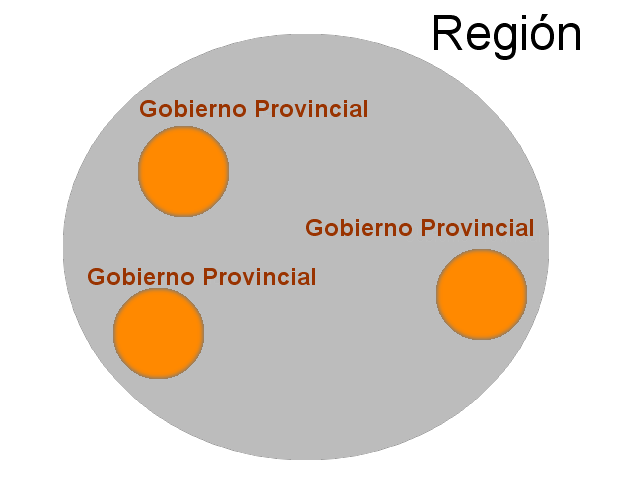
\includegraphics[scale=0.4]{regionProvincia.png}
\end{figure}

De �sta forma, se tiene un mejor control de los datos y los modelos de las diferentes provincias, ademas de distribuir la ejecuci�n de una misma regi�n.

La comunicaci�n entre $Estaciones$ $Centrales$ pude realizarse por diferentes medios de comunicaci�n, ya sea por gsm o por internet por ejemplo y eso estar� descripto en la descripci�n de funcionalidad del componente responsable de esa comunicaci�n. Esta comunicaci�n se realizar� mediante mensajes de control que permitan a una Estaci�n central, pedir resultados parciales de un modelo, o pedir informaci�n de ciertos sensores a otras Estaciones Centrales regionales.

\section{Estructura}

Para poder cumplir con estos requerimientos, como se dijo se deber�n agregar estaciones centrales de forma distribuida a lo largo de todo el pais.
Pero con la restricci�n de que exista a lo sumo una por provincia. Sumado a esto cada una de estas EC provinciales (ECP) tendran un sistema de
monitoreo (SMP) muy parecido al original s�lo que tendr� las componentes fundamentales, las que son pertinentes al manejo provincial.

Esto no cambia, sin embargo, que exista una estacion central con todas las funcionalidades originales y tambien su sistema de monitoreo correspondiente.

Otro gran cambio que se realiza en cuanto a la forma de obtenci�n de datos de una TR es que la EC o ECP que necesite los datos de dicha TR trandra que
suscribirse y estas cada vez que tengan un nuevo dato lo enviar�n a todos los suscriptos (publish/subscribe).
Este mecanismo tiene el limite del control provincial, las ECP s�lo se podran suscribir a las TR que esten en la regi�n de la provincia. Si llegaran a necesitar
un dato de una TR en la misma regi�n pero en otra provincia, deberan suscribirse a los datos de dicha TR a trav�s de la ECP que los controle.

El mecanismo de suscripci�n y publicaci�n de datos en una TR y en una EC o ECP ser�n polimorficos, logrando de esta forma transparencia a la hora de notificar
y/o suscribirse a los datos.

Otro detalle importante en cuanto a la suscripci�n de estos datos, se podr�n hacer pidiendo un subconjunto de los sensores que posea la TR correspondiente.
Esta a su vez sabra responder que tipo de sensores tiene presentes.

El �ltimo cambio que se realiza es que no s�lo se podra una ECP suscribir a otra para pedir datos de alguna TR en su provincia con ciertos sensores, si no 
que tamiben se podr� suscribir a datos parcial o totalmente calculados por un modelo en la EC o ECP.


